% !TeX root = ../msc-thesis.tex
\documentclass[../msc-thesis.tex]{subfiles}

\begin{document}

\chapter{Non linear optimization and infill criteria}

When dealing with a non linear problem, such as in \autoref{soc:optproblem}, 
typically it is resorted to classical solvers (e.g. SQP, trust-region-dogleg, 
genetic algorithms, simulated annealing, etc.) to obtain its solution, 
depending on the nature of the NLP (e.g. presence of discontinuities, whether 
or not the function is differentiable, etc.).

There is a entire field of study dedicated to find these NLP solutions with 
\kriging surrogates. In the works of \textcite{Jones2001, Sasena2002, 
Forrester2008, Alexandrov2000}, there are entire discussions and frameworks 
on how to solve non linear problems and comparisons of several metrics 
involved in the optimization process with metamodels.

The premise of performing a optimization using surrogates is that the model 
to be optimized is too time consuming or computationally expensive to be 
solved with classical solvers. To circumvent this, the following steps are 
proposed: 

\begin{enumerate}
    \item Build an approximation model with \kriging surrogates using a 
    limited number of initial samples. This approximation is a ``generalistic'' 
    enough representation of the real model; \label{inf2}

    \item Perform an optimization of the approximation model using classical NLP
    solvers and an infill criteria. The surrogate model reduces the 
    ``search area'' needed by the solver; \label{inf2}

    \item Compare the surrogate optimum found in step \ref{inf2} with the 
    result from original model. In other words: feed the results from the 
    \kriging metamodel optimum into the original model and see if they are 
    close enough; \label{inf3}

    \item If the optimum from the metamodel is close enough (based on a 
    chosen metric) to the original model, then this may be the true optimum. 
    Otherwise, update the \kriging model by introducing the value found and 
    return to step \ref{inf2}; \label{inf4}
    
\end{enumerate}

This process is basically ``filling holes'' (hence the name \textit{infill}) 
in our \kriging metamodel until original model optimum is found. To illustrate 
this in the simplest way, suppose a complex process that we need to optimize 
that is represented by the following function:

\begin{equation*}
    f(x) = -\cos(x) - e^{\frac{x}{20}} + 5
\end{equation*}

Assuming that we only have three initial points sampled from this model 
function, we build our \kriging model. As can be seen in 
\autoref{fig:infill_init}.

\begin{figure}[htb]
    \caption{\label{fig:infill_init}Initial plot of our complex model. The 
    solid blue line represents the function behavior. The dashed line is the 
    \kriging metamodel of the three sampled points (red circles) available.}
    \centering
    \def\svgwidth{\columnwidth}
    \input{../images/infill_init.pdf_tex}
    \fonte{Author.}
\end{figure}

When applying an optimization solver on the \kriging model, we get a new 
optimal value for $x$ near 7.8 (3.47 for $f(x)$ when we consult the original 
model). Now, we include these values of $(x, f(x))$ in the sample and rebuild 
the \kriging metamodel. The result is shown \autoref{fig:infill_1}. We keep 
repeating this procedure until we get the result in \autoref{fig:infill_2}.

\begin{figure}[htb]
    \caption{\label{fig:infill_1}The \kriging model after one update.}
    \centering
    \def\svgwidth{\columnwidth}
    \input{../images/infill_1.pdf_tex}
    \fonte{Author.}
\end{figure}

\begin{figure}[htb]
    \caption{\label{fig:infill_2}The \kriging model after four updates. 
    Notice how the \kriging model adjusts to the true function.}
    \centering
    \def\svgwidth{\columnwidth}
    \input{../images/infill_2.pdf_tex}
    \fonte{Author.}
\end{figure}

This example is a trivial one because the problem involves a single input 
variable and infill criteria is the own \kriging prediction of the model. As 
discussed in \textcite{Jones2001}, this criteria has its pitfalls if used 
without other precautions.

\textcite{Caballero2008} presented an algorithm, based on the ``method 2'' 
in the work of \textcite{Jones2001}, referred as a gradient matching 
technique where the gradient of the surrogate is forced to match with 
the true function gradient, this is done through trust-region approach to 
ensure local convergence which was proven in the work of 
\textcite{Alexandrov2000}. The basic idea of this approach is: minimize the 
NLP problem metamodel, consult the original function at the minimum found in 
the metamodel, update the sample matrix used to build the surrogate. Repeat 
this until a convergence criteria is met. The flowchart depicting the 
whole procedure is defined in \autoref{fig:caballeroflowchart}. For detailed 
explanation of each step of the proposed algorithm, one must refer to 
\textcite{Caballero2008} and \textcite{Alves2018}.

\begin{figure}[htb]
    \caption{Flowchart of \textcite{Caballero2008} algorithm, translated to 
    Python by the author of this work and implemented within \mtc.}
    \centering
    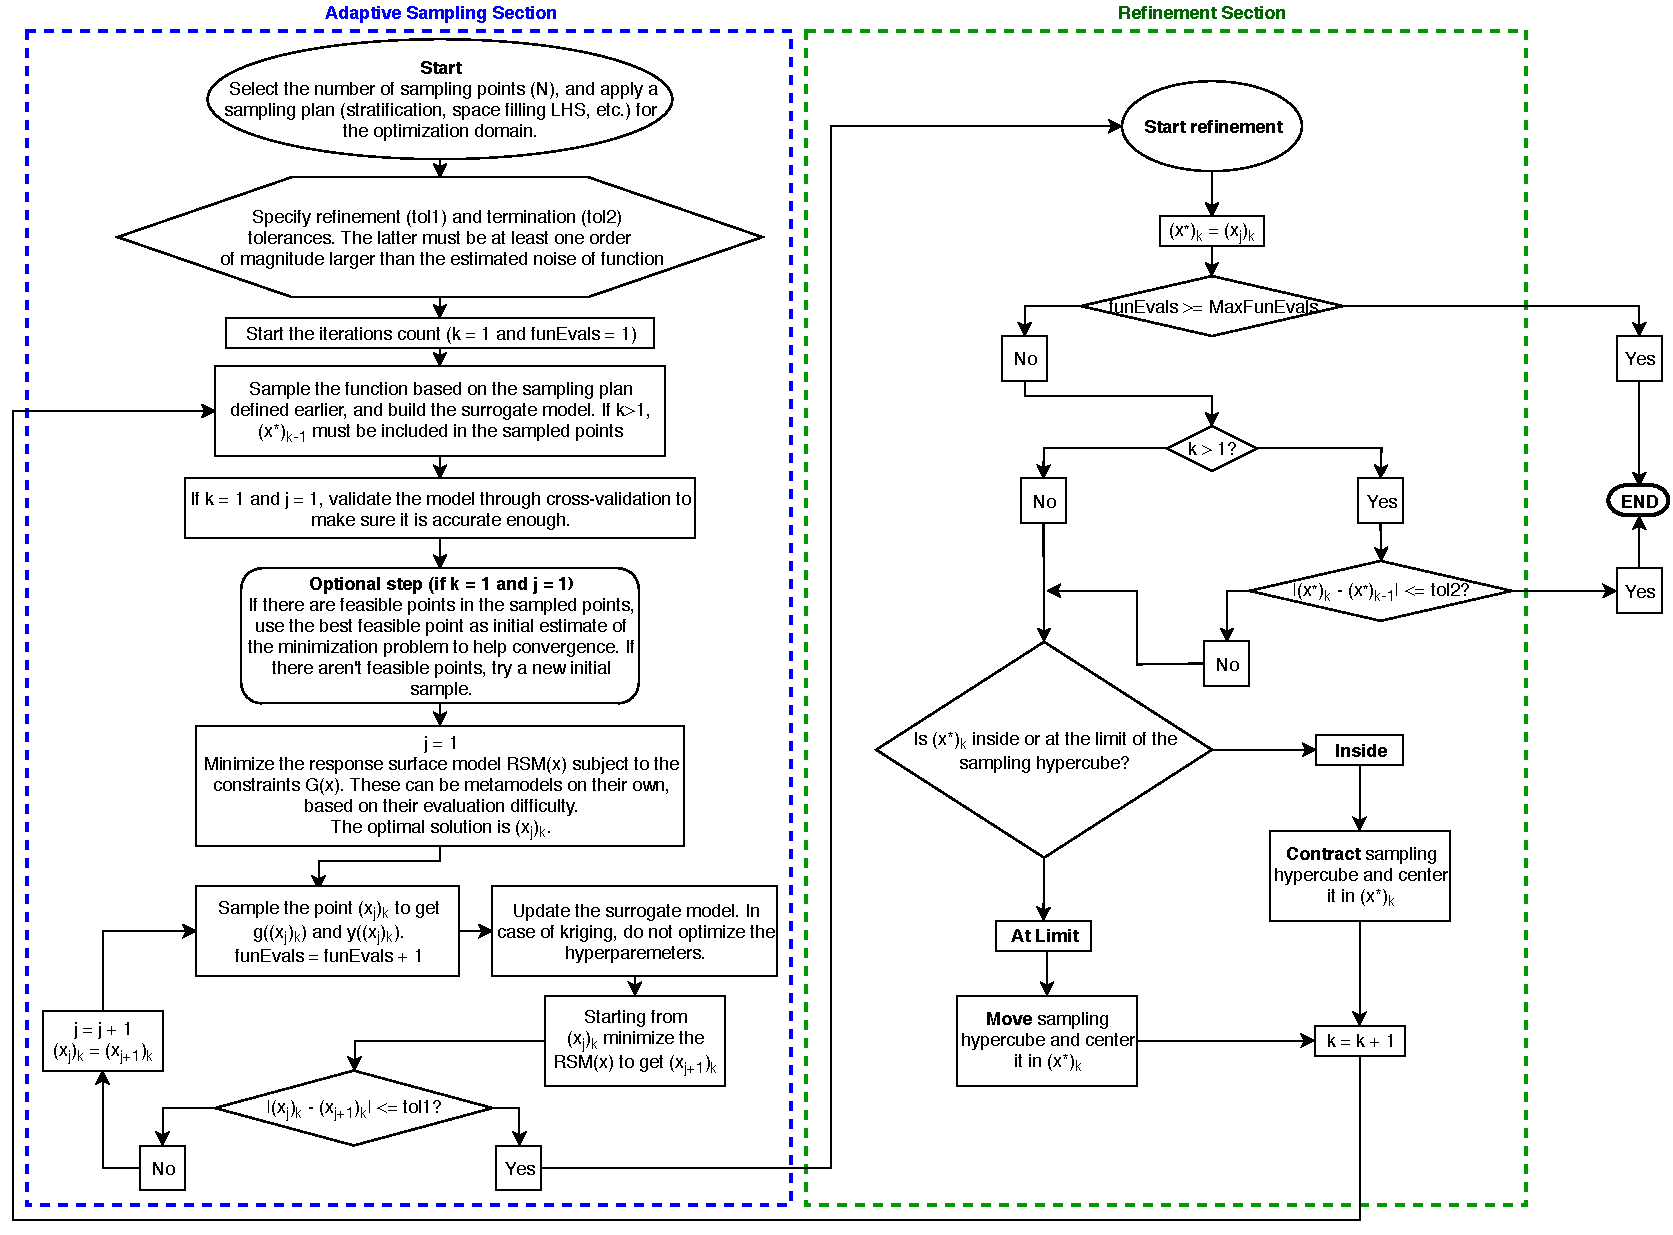
\includegraphics[angle=90, scale=0.8]
    {caballero_flowchart_final.pdf}
    \label{fig:caballeroflowchart}
    \fonte{\textcite{Alves2018}}
\end{figure}

This approach was implemented as a procedure of the Python package 
\textit{surropt} (from \textit{Surrogate Optimization}). It uses as 
internal NLP solver a Python wrapper authored by \textcite{Cyipopt2019} of 
the well-established \textit{IpOpt} package \cite{Wachter2006}. The 
\textit{surropt} package is found on \url{https://github.com/feslima/surropt}.

\end{document}